%% Style 52
% CHOMSKY

\cxset{
 name=CHAPTER,
 numbering=arabic,
 number font-size=\large,
 number before={},
 number position=rightname,
 chapter spaceout=soul,
 chapter color={black!80},
 chapter font-size=\large,
 chapter before=\rule[3pt]{\textwidth}{0.4pt}\par\hfill,
 number after=,
 chapter after=\hfill\hfill\par\vspace*{-3pt}\rule[3pt]{\textwidth}{0.4pt}\par,
 number color=\color{black!80},
 title font-family=\bfseries,
 title font-color=\color{black!80},
 title font-weight=,
 title font-size=\Huge,
 title before=\hfill,
 title after=\hfill\hfill,
 title beforeskip=\vspace*{1cm},
 title afterskip=\vspace*{1.5cm},
 epigraph width=0.85\textwidth,
 epigraph align=center,
 header style=empty}

\chapter{Introduction to Style Fifty Two}

\epigraph{In the late forties \ldots\ it seemed to many that the conquest of syntax finally lay open before the profession. At the beginning of the fifties confidence was running high.}{H. Allan Gleason}

\section{Looking for Mr. Goodstructure}
This is an unusual book with a rather unique style. The vertical rule is simple and breaks the monotony of a book that is heavy on text.
\begin{figure}[ht]
\centering
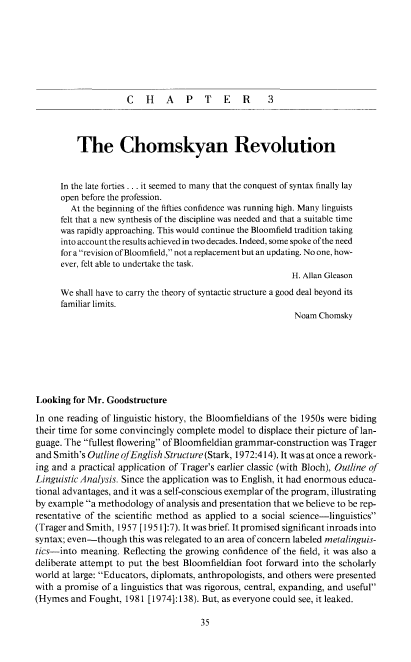
\includegraphics[width=0.35\textwidth]{./chapters/chapter52}
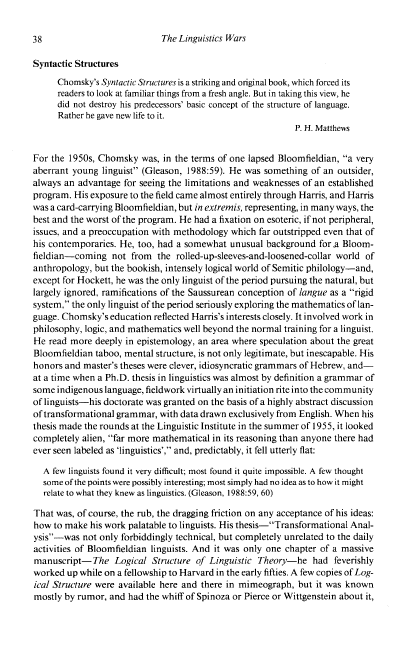
\includegraphics[width=0.35\textwidth]{./chapters/chapter52a}
\caption{Style 50 from the Oxford Handbook of Cuneiform Culture.}
\end{figure}

This style is very modern and typical of many computer books. The difficulty is in integrating all the page elements to make it work flawlessly.

